\documentclass[xcolor={dvipsnames},pdf, hyperref={colorlinks=true, citecolor=ForestGreen, linkcolor=BlueViolet, urlcolor=Magenta}]{beamer}
\usetheme{Frankfurt}  
\usecolortheme{whale}
\usepackage{tikz} 
\usepackage{graphicx}
\usepackage{dsfont}
\usepackage{hyperref}
\usepackage{alltt}
\usepackage{enumerate}
\usepackage{amsthm}
\theoremstyle{definition}
\newtheorem{exmp}{Example}[section]
\usepackage{verbatim}               % useful for \begin{comment} and \end{comment}
\usepackage{eurosym}                % used for euro symbol
\usepackage{caption} 
\usepackage{graphicx}
\usepackage{adjustbox}
\graphicspath{{Figures/}}
\usepackage{subcaption}
\usepackage{color}
\usepackage{float}
\usepackage{amssymb}
\usepackage{sgamevar}
\usepackage{remreset}% tiny package containing just the \@removefromreset command
\makeatletter
\@removefromreset{subsection}{section}
\makeatother
\setcounter{subsection}{1}



\newcommand{\defn}[1]{\textbf{#1}}


%Instructor version
\newcommand{\blank}[0]{}
\newcommand{\ddp}[1]{{\textcolor{ForestGreen}{#1}}} 
\newcommand{\dd}[1]{{\underline{\textcolor{ForestGreen}{#1}}}}

%Student version
%\newcommand{\blank}[0]{\vspace{2em}}
%\newcommand{\dd}[1]{\underline{\hspace{3cm}}} 
%\newcommand{\ddp}[1]{}

\addtobeamertemplate{navigation symbols}{}{%
	\usebeamerfont{footline}%
	\usebeamercolor[fg]{footline}%
	\hspace{1em}%
	\insertframenumber/\inserttotalframenumber
}

\section{The Labor Force}

%% preamble
\title{The Labor Force and Unemployment}
\author{David A. D\'iaz}
\institute{UNC Chapel Hill}
\date{}

\AtBeginSection[] %Section links on slides

\begin{document} 
	
	\begin{frame}
		
		\titlepage
		
	\end{frame}


\begin{frame}{The Labor Force}
	\begin{itemize}
	\item There are three categories the ``working population'' can be placed in:
	
	\begin{enumerate}
		\item Employed (\textbf{E}): Those who work as paid employees, worked in their own business, or worked as unpaid workers in a family business. Includes part-time and full-time workers and those on temporary leave.
		\item Unemployed (\textbf{U}): Those who are not employed, are available for work, and have tried to find employment during the previous four weeks.
		\item Not in the labor force (\textbf{O}): Everyone else -- full-time students, retirees, etc.
	\end{enumerate}
	
	\item \defn{Labor Force (LF):} The total number of workers = E + U
	


\end{itemize}
\end{frame}

\begin{frame}{The Labor Force}
\begin{itemize}


	\item \defn{Labor Force (LF):} The total number of workers = E + U
	
	\item Not included in P:
	\begin{itemize}
		\item Military members (only counting the civilian population)
		\item Institutionalized individuals (e.g., in jail)
		\item Individuals who are less than 16 years old
	\end{itemize}
\end{itemize}
\end{frame}

\begin{frame}{The Labor Force}
\begin{itemize}
	\item \defn{Labor-force participation rate (LFPR):} \% of the adult population that is in the labor force 
	
	\[LFPR = \frac{LF}{P} = \frac{E + U}{E + U + O}\]
	
\end{itemize}
\end{frame}


\begin{frame}{The Labor Force}
\begin{exmp}
	\scriptsize
Suppose there are 12,500 individuals over age 16 in Waxhaw. Of these individuals,

\begin{itemize}
	\item 3,500 work full-time in the private sector \ddp{\pause E}
	\item 2,000 work full-time in the public sector (non-military) \ddp{\pause E}
	\item 2,000 work part-time in the private sector \ddp{\pause E}. Of these part time workers, 20\% are working part-time for economic reasons and would prefer full-time work.
	\item 1,500 individuals were laid off 6 months ago due to a plant closing. Of these laid off individuals, 1,000 have actively sought work since being laid off, while 500 searched for work immediately after being laid off, but not in the last four weeks. \ddp{\pause 800 U, 700 O}
	\item 1,000 do not have formal employment and instead choose to stay home to care for children \ddp{\pause O}
	\item 2,500 are retired from work and neither have nor seek employment. \ddp{\pause O}
\end{itemize}
 What is the labor force participation rate?
\ddp{\pause $LFPR = LF/P = (E + U)/P = 8,500/12,500 = 68\%$}
\end{exmp}
\end{frame}

	\begin{frame}{Trends in the US Labor Force}
	\begin{itemize}
		\item Decline in LFPR for males particularly steep for those $\sim$ 65 years or older. 
		\item Dramatic increase in LFPR of women in the last 50 years. Particularly steep among married women.
	\end{itemize}	
	\begin{figure}
		\centering
		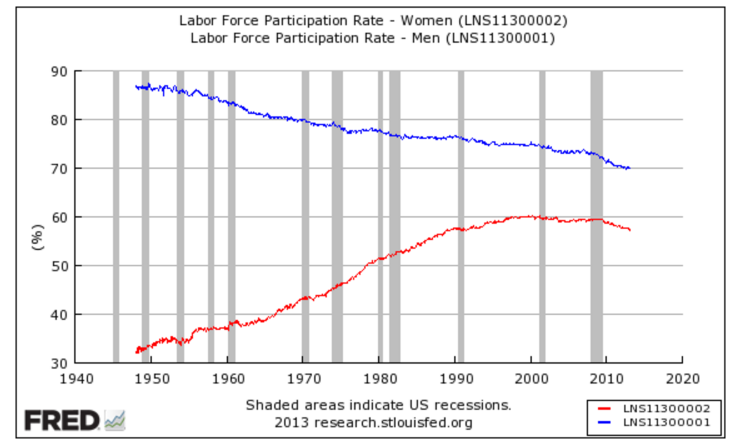
\includegraphics[scale=.8]{01B_5.png}
		\caption{LFPR by Sex, 1948 - 2015}
	\end{figure}
\end{frame}

	\begin{frame}{Trends in the US Labor Force}
	\begin{itemize}
		\item Tough to explain fall in the LFPR among prime-age males.
	\end{itemize}
	\begin{figure}
		\centering
		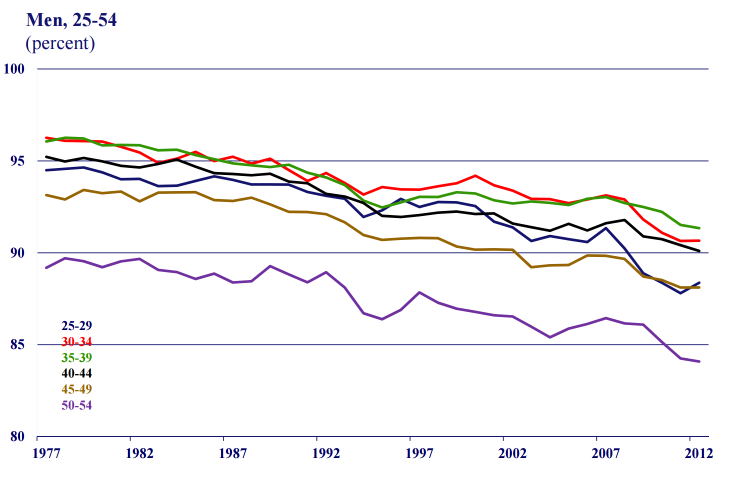
\includegraphics[scale=.8]{01B_13.png}
		\caption{Male LFPR by Age, 1977-2012}
	\end{figure}
\end{frame}

	\begin{frame}{Trends in the US Labor Force}
	\begin{figure}
		\centering
		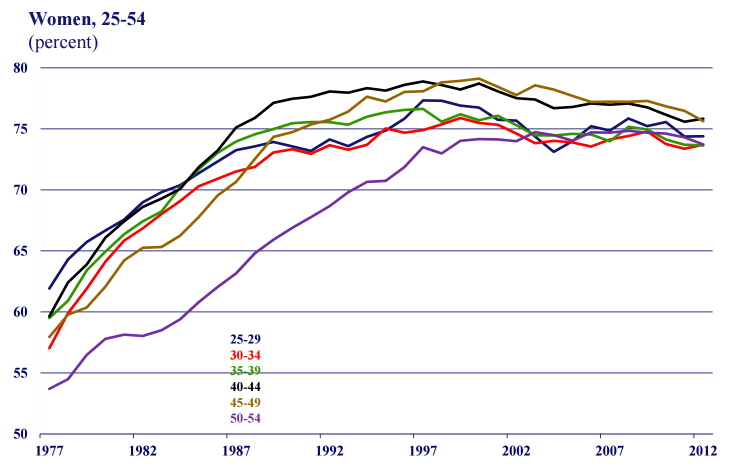
\includegraphics[scale=.9]{01B_14.png}
		\caption{Female LFPR by Age, 1977-2012}
	\end{figure}
	
\end{frame}


	\begin{frame}{Trends in the US Labor Force}
	\begin{itemize}
		\item LFPR of those in retirement years has increased recently.
	\end{itemize}
	\begin{figure}
		\centering
		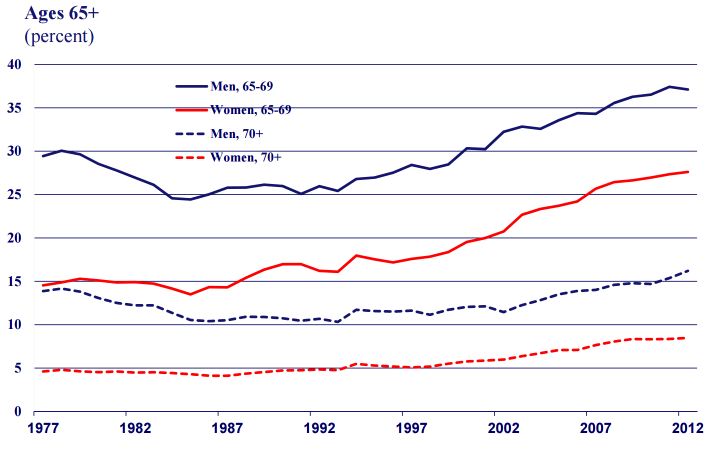
\includegraphics[scale=.8]{01B_15.png}
		\caption{LFPR in Retirement Years, 1977-2012}
	\end{figure}
\end{frame}


	\begin{frame}{Trends in the US Labor Force}
	\begin{figure}
		\centering
		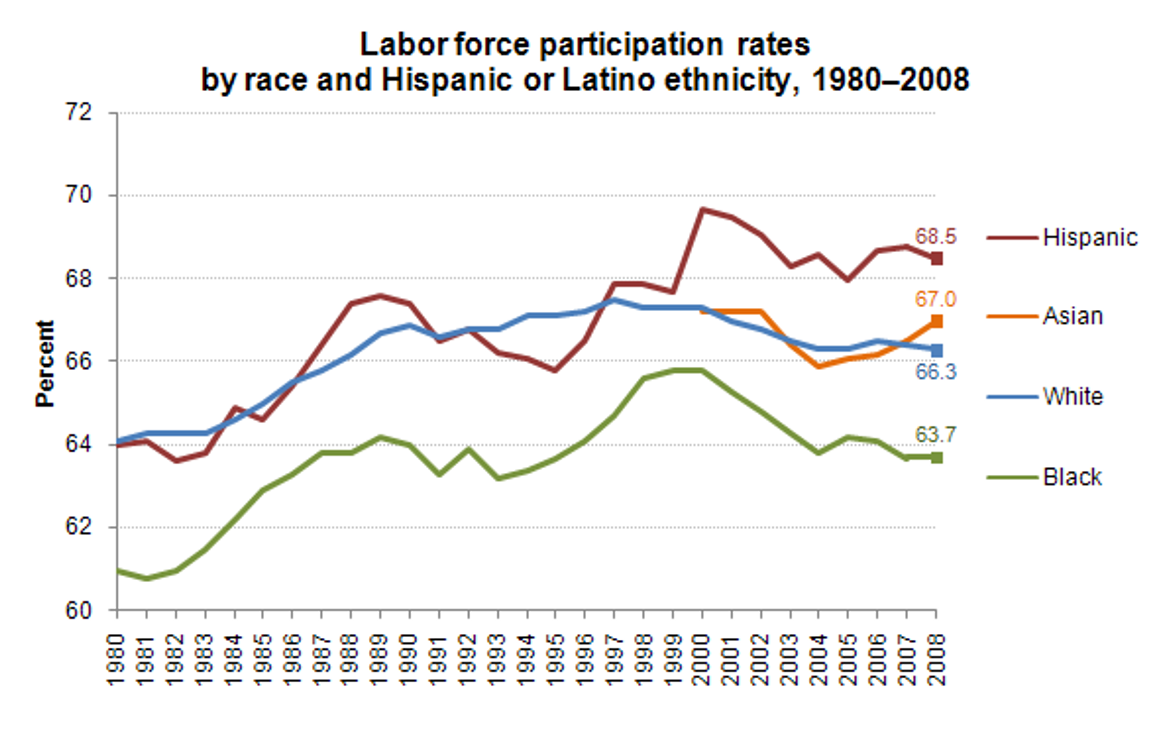
\includegraphics[scale=.6]{01B_7.png}
		\caption{LFPR by Race/Ethnicity, 1980-2008}
		\item 
	\end{figure}
	
\end{frame}

\section{Unemployment}

\begin{frame}{Unemployment}
\begin{itemize}
	 \item \defn{Unemployment rate (UR):} \% of the labor force that is unemployed  
	
	\[UR = \frac{U}{LF} = \frac{U}{E + U}\]
\end{itemize}

\begin{exmp}
	What is the unemployment rate in Waxhaw?
\end{exmp}

	\ddp{\pause $UR= U/LF = 1000/8,500 = 11.8\%$}

\end{frame}

\begin{frame}{US Unemployment Trends}
	\begin{figure}
		\centering
		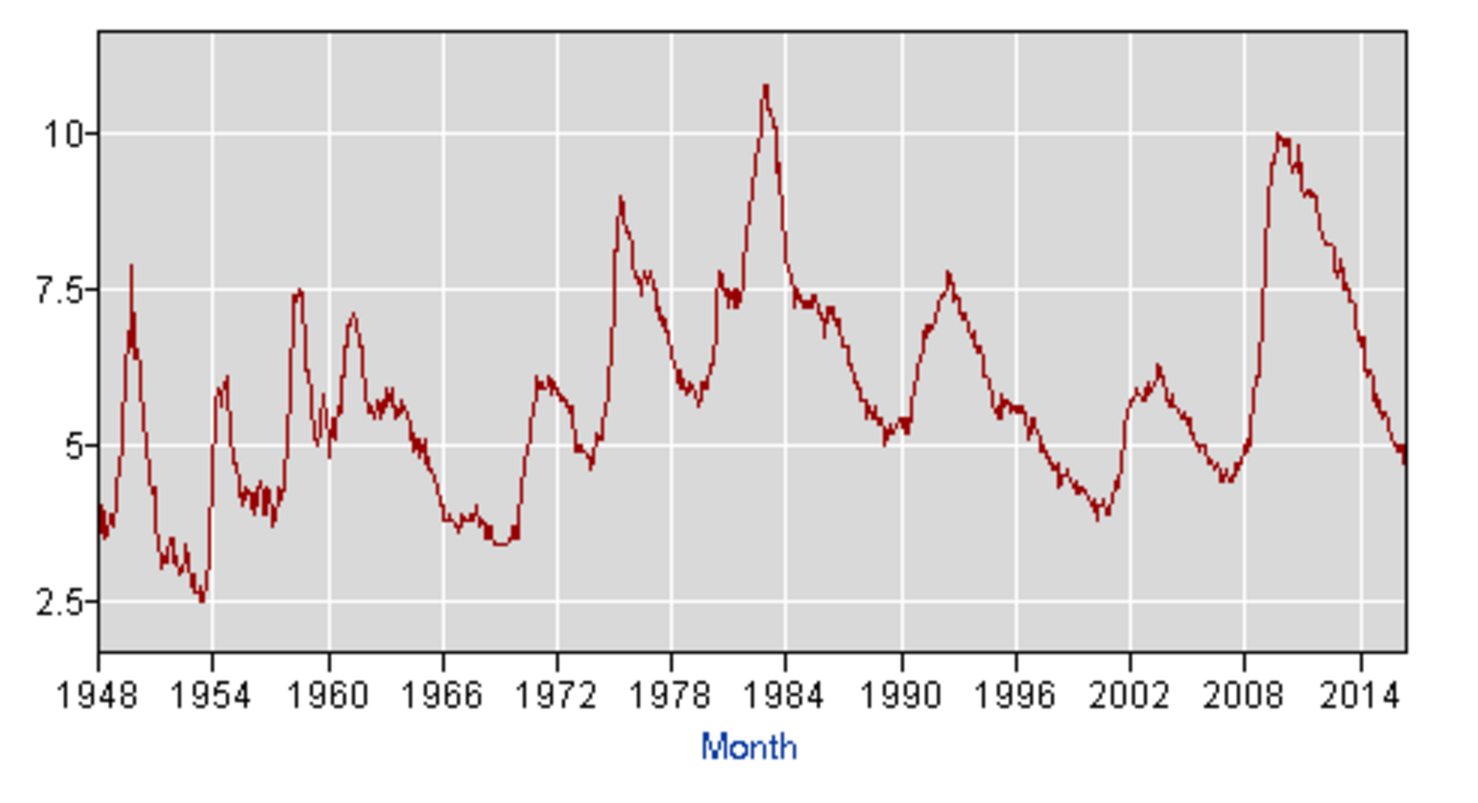
\includegraphics[scale=.5]{01C_11.png}
		\caption{Unemployment Rate, 1947-2016}
	\end{figure}
\end{frame}

\begin{frame}{US Unemployment Trends}
	\begin{figure}
		\centering
		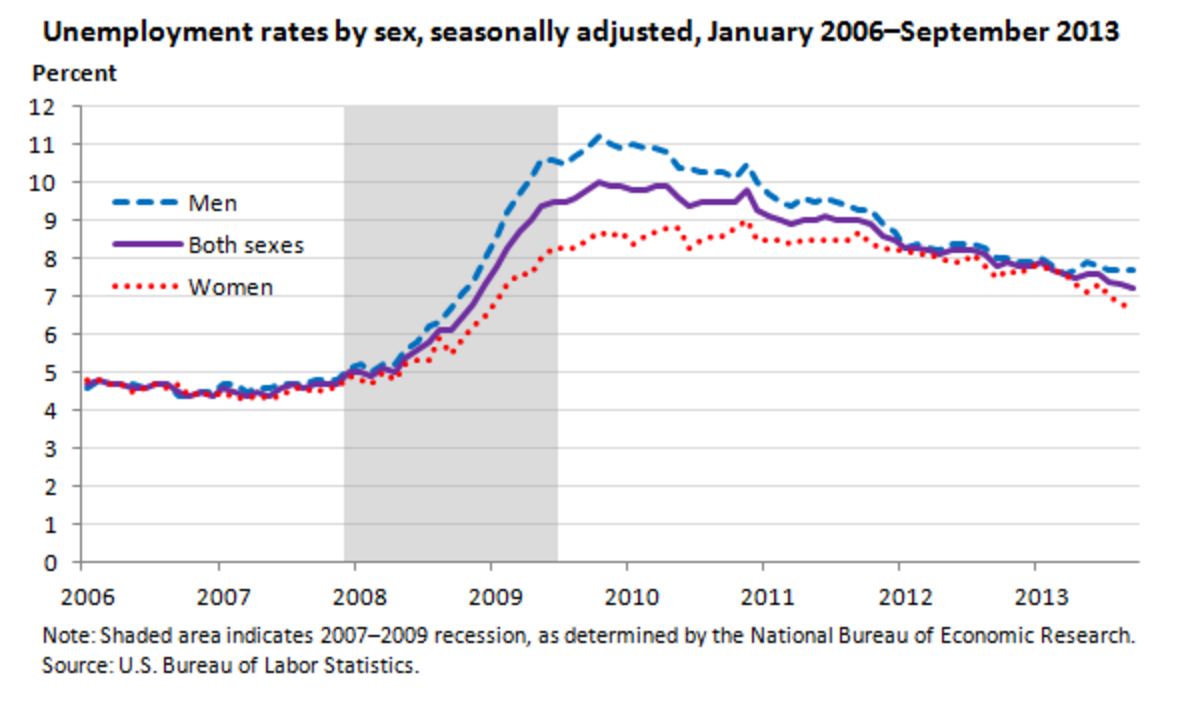
\includegraphics[scale=.6]{01C_3.png}
		\caption{Unemployment Rate by Sex, 2006-2013}
	\end{figure}
\end{frame}

\begin{frame}{US Unemployment Trends}
	\begin{figure}
		\centering
		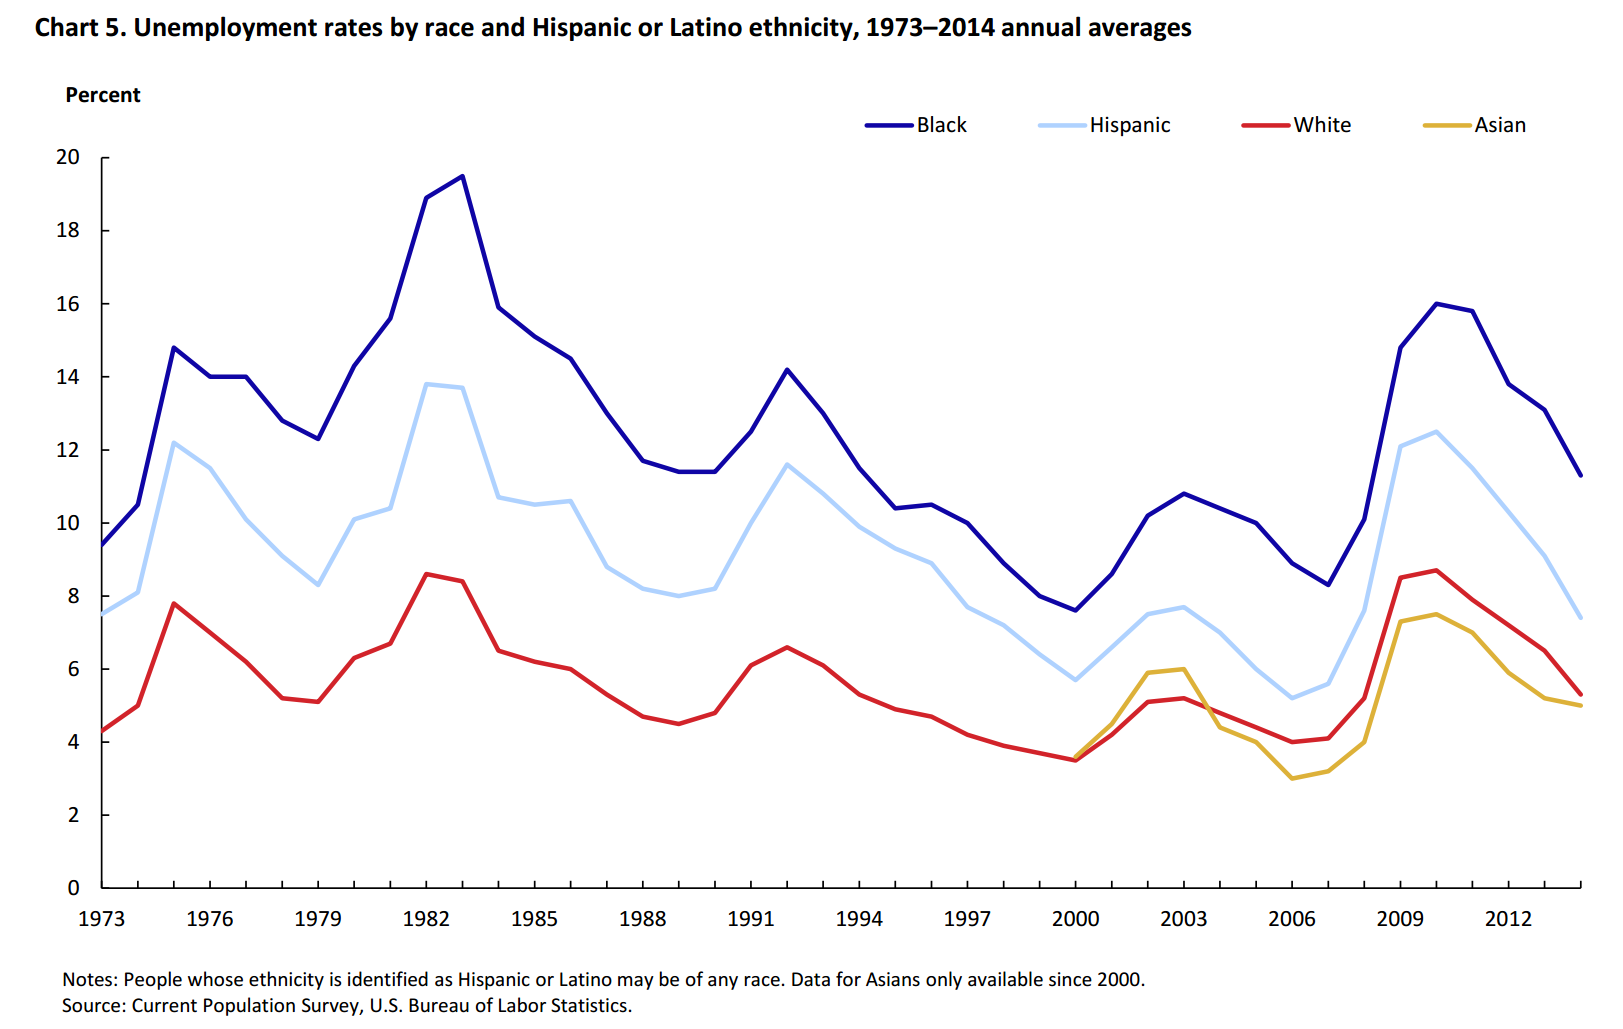
\includegraphics[scale=.5]{01C_1.png}
		\caption{Unemployment Rate by Race, 1973-2014}
	\end{figure}
\end{frame}

\begin{frame}{US Unemployment Trends}
	\begin{figure}
		\centering
		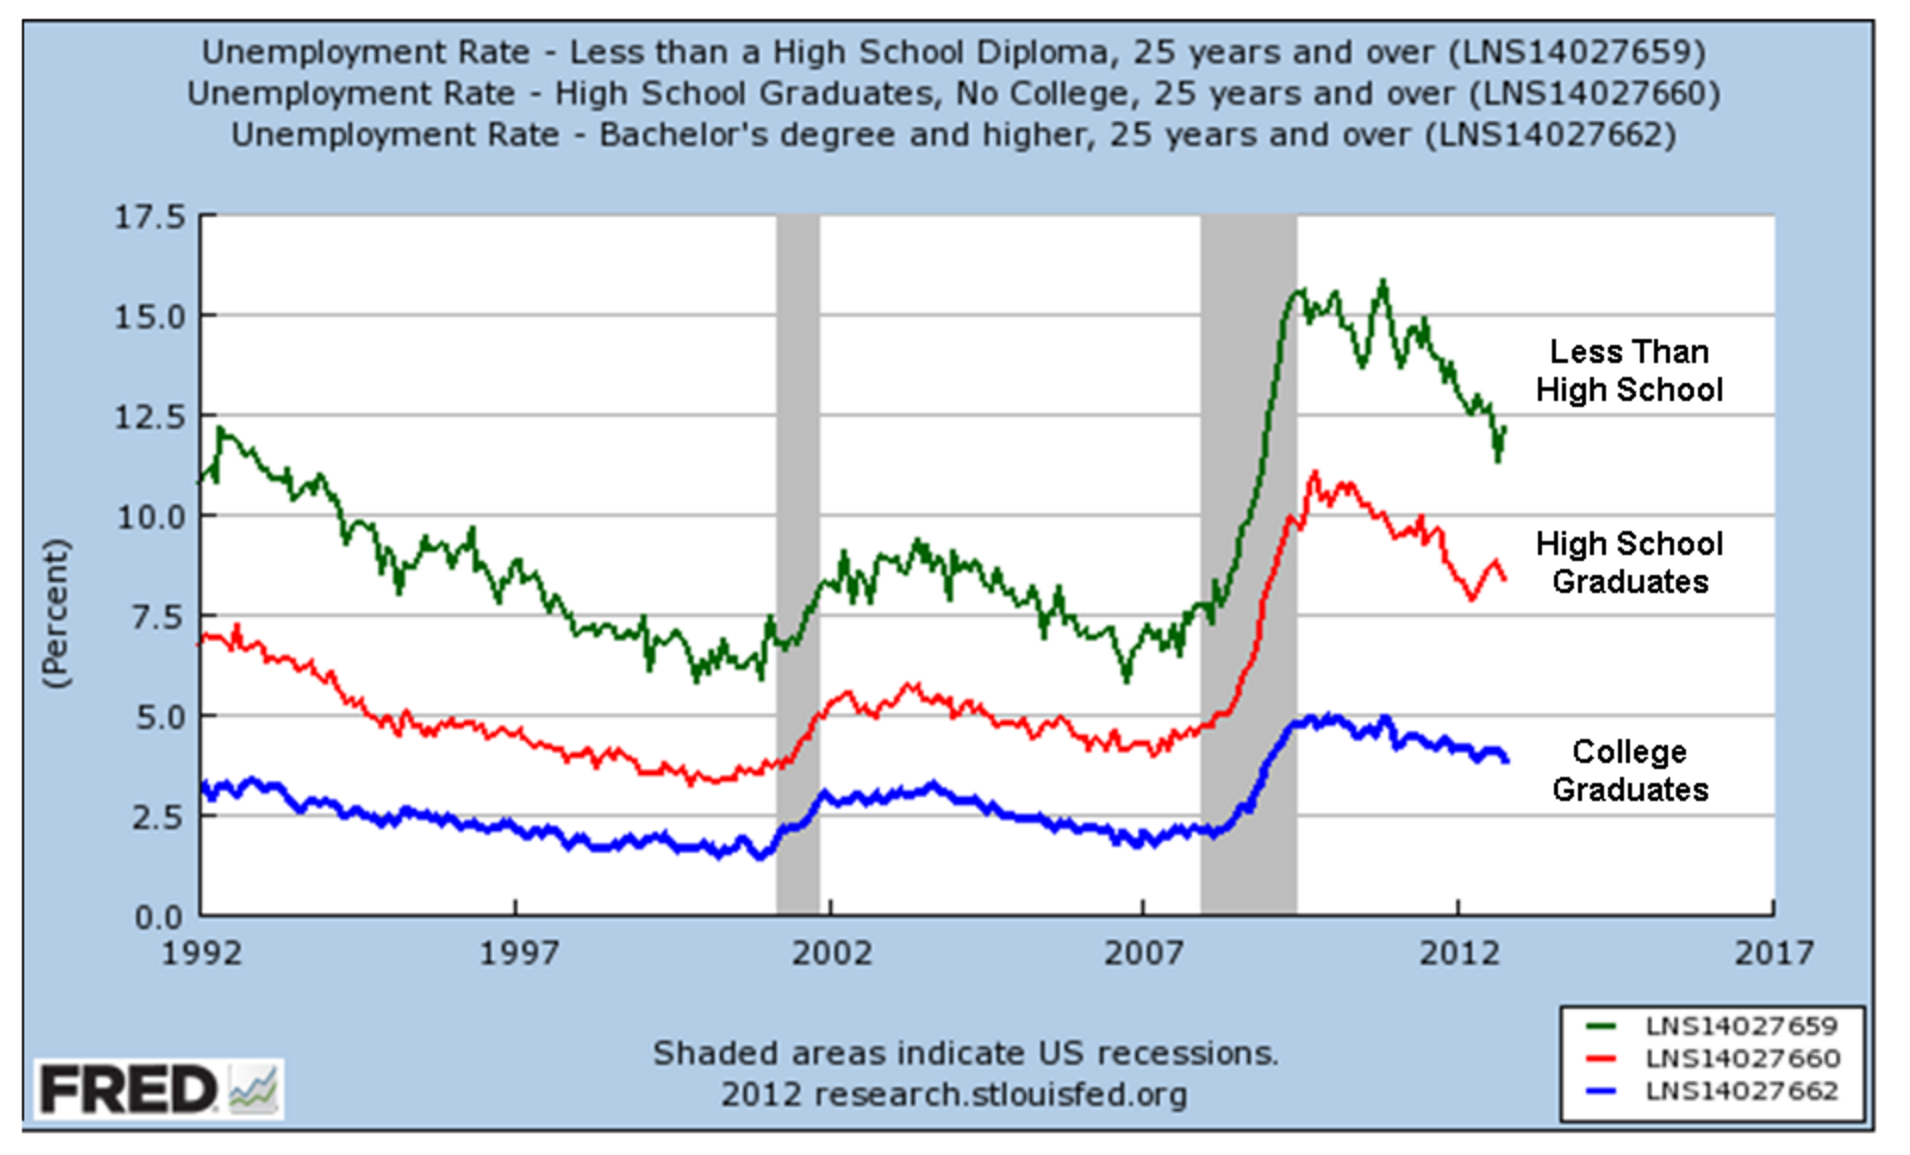
\includegraphics[scale=.4]{01C_2.png}
		\caption{Unemployment Rate by Education, 1992-2012}
	\end{figure}
\end{frame}

\begin{frame}{Unemployment}
\begin{exmp} 
	\scriptsize
	In each of the following, what happens to the unemployment rate? In each case does the unemployment rate give an accurate impression of what is happening in the labor market?
	\begin{enumerate}
		\item Sue lost her job, and begins looking for a new one. 
		\item Jon, a steelworker who has been out of work since his mill closed last year, becomes discouraged and gives up looking for work. 
		\item Sam, the sole earner in his family of 5, just lost his \$80,000 job as a research scientist. Immediately, he takes a part-time job at McDonald's until he can find another job in his field.
	\end{enumerate}
\end{exmp}
\scriptsize
\ddp{\pause \#unemployed increases, LF stays the same. Unemployment rate increases. Accurately reflects that labor market \\
\pause \#Unemployed and \# in labor force decreases. Overall unemployment rate falls. Does not give an accurate description of labor market \\
\pause No change in the unemployment rate. Does not accurately reflect changes in labor market}
\end{frame}


\begin{frame}{Unemployment}
\begin{itemize}
	\item The task of determining whether someone is unemployed or simply not in the labor force makes measuring the true amount of unemployment in an economy difficult. 
	\item Is the unemployment rate a good measure of joblessness? What's missing? 
\end{itemize}
\end{frame}

\begin{frame}{Unemployment}
	\begin{itemize}
	\item Discouraged/marginally attached workers are considered out of the labor force
\end{itemize}
\begin{figure}
	\centering
	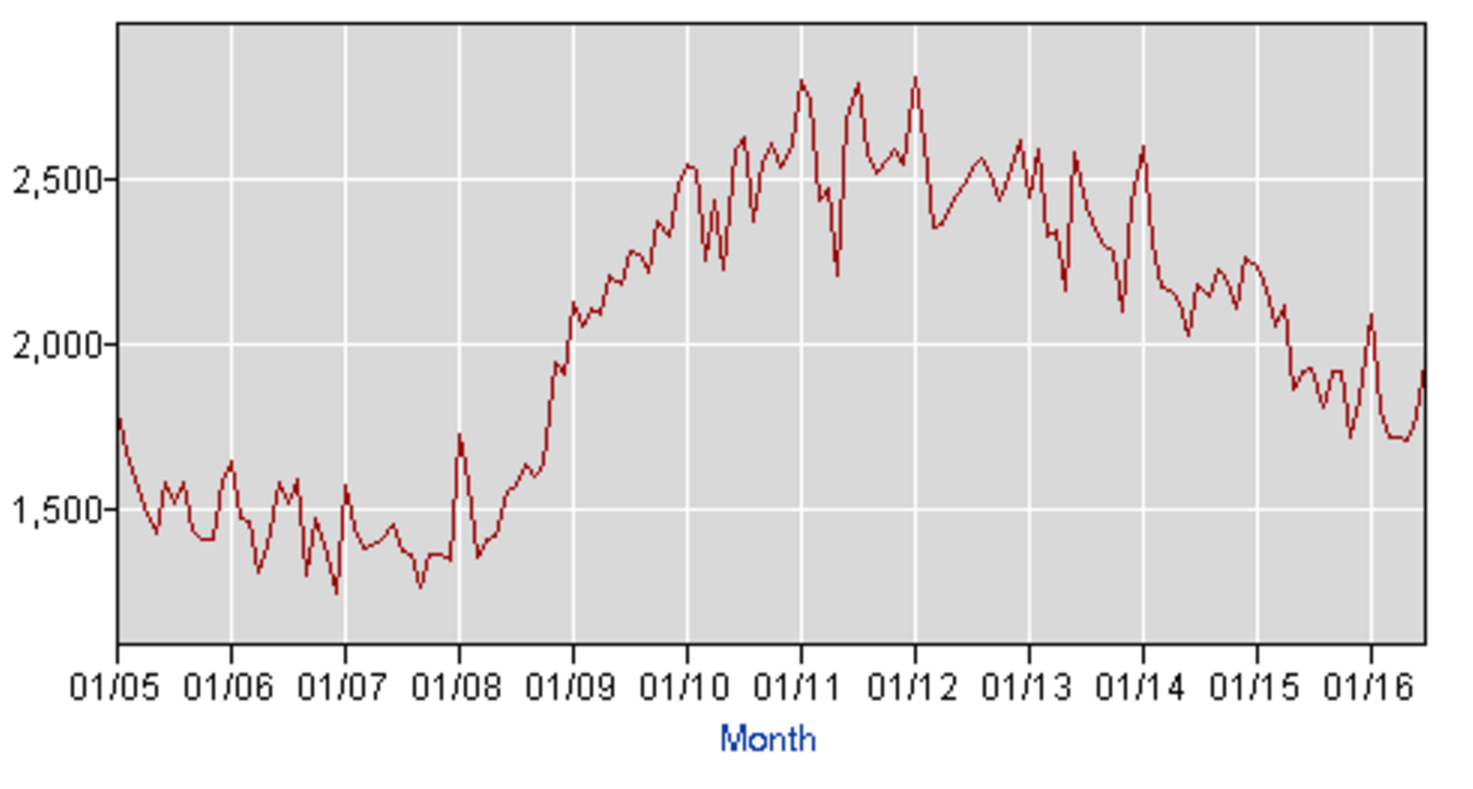
\includegraphics[scale=.4]{01C_10.png}
	\caption{Marginally Attached Workers (thousands), 2005-2016}
\end{figure}

\end{frame}


\begin{frame}{The Unemployment Rate: Issues}
	\begin{itemize}
		\item Underemployment is not taken into account
		\begin{itemize}
			\item Highly skilled workers in low paying jobs
			\item Highly skilled workers in low skill jobs  
			\item Part-time workers who would prefer to be full time.
		\end{itemize}
	\end{itemize}
	\begin{figure}
		\centering
		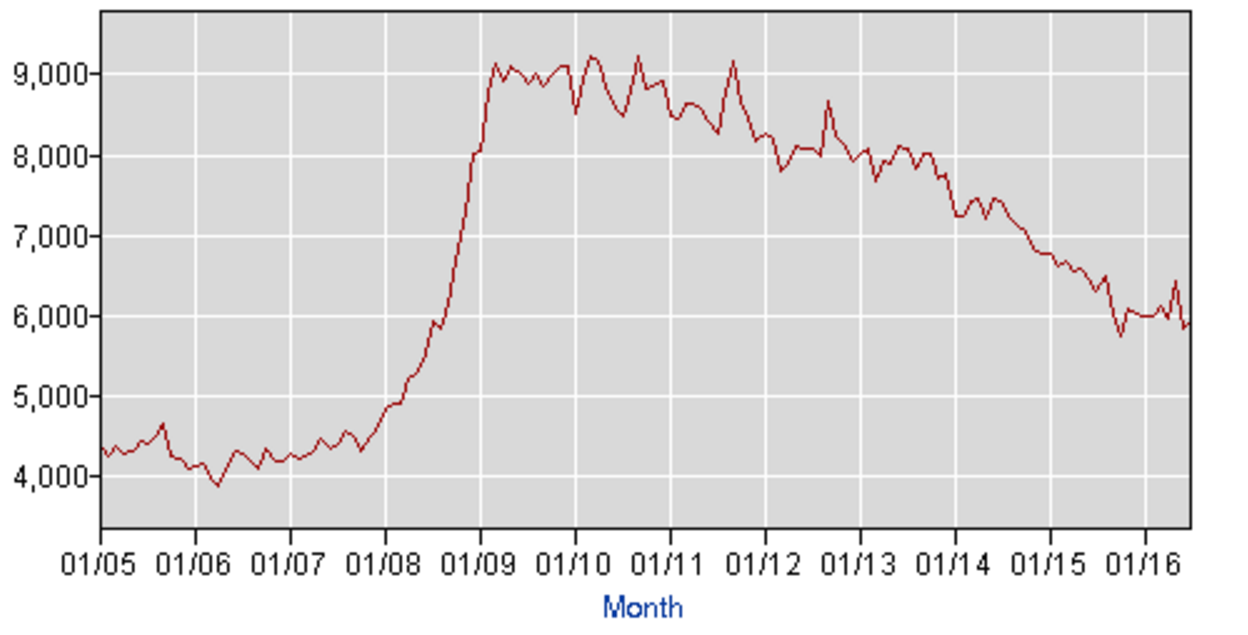
\includegraphics[scale=.4]{01C_12.png}
		\caption{Part time Workers for Economics Reasons (thousands), 2005-2016}
	\end{figure}
\end{frame}

\begin{frame}{The Unemployment Rate: Issues}
	\begin{itemize}
		\item Length of unemployment not taken into account
		\begin{itemize}
			\item Short spells indicate labor market fluidity
			\item Long spells indicate more serious issues
			\item Upward trend in the fraction of the unemployed who had been without work more than 26 weeks 
			\item More pronounced during recent recession
		\end{itemize}
		\begin{figure}
			\centering
			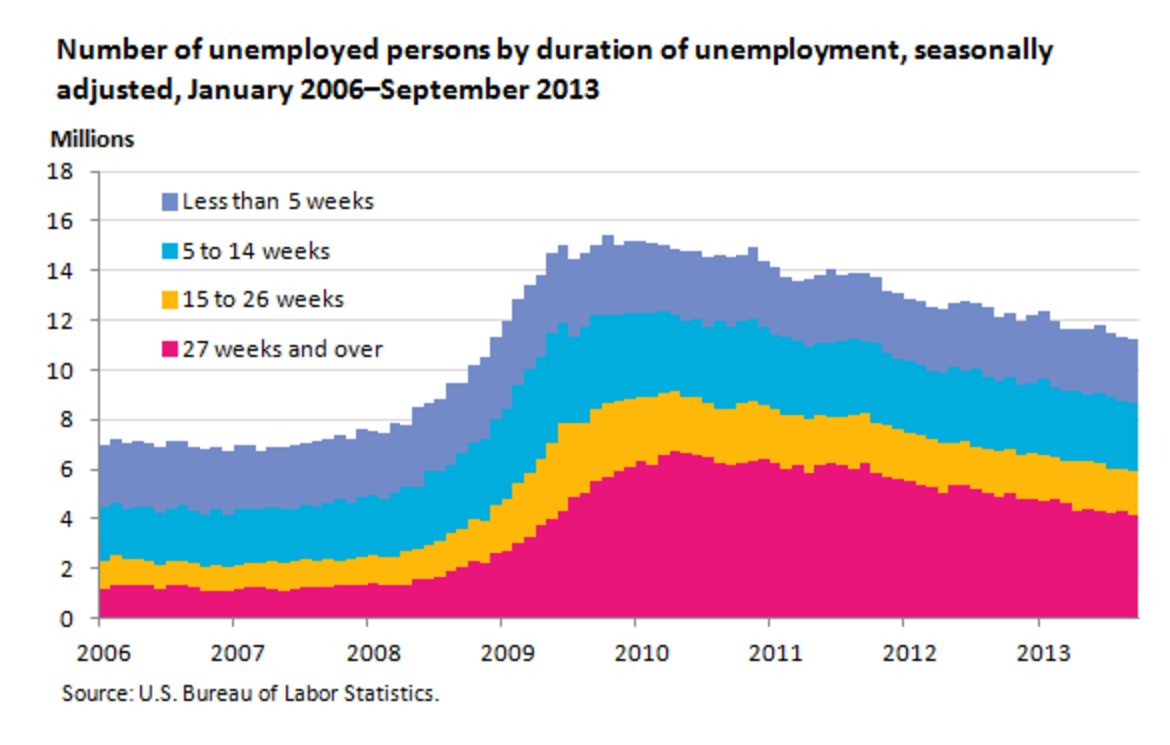
\includegraphics[scale=.5]{01C_4.png}
			\caption{Unemployment Spells, 2006-2013}
		\end{figure}	
	\end{itemize}
\end{frame}	

\begin{frame}{The Unemployment Rate: Issues}
	\begin{itemize}
		\item These factors are more severe during recessions
		\item Unemployment rate may understate the depths of recessions and state of economic hardship 
	\end{itemize}
	\begin{figure}
		\centering
		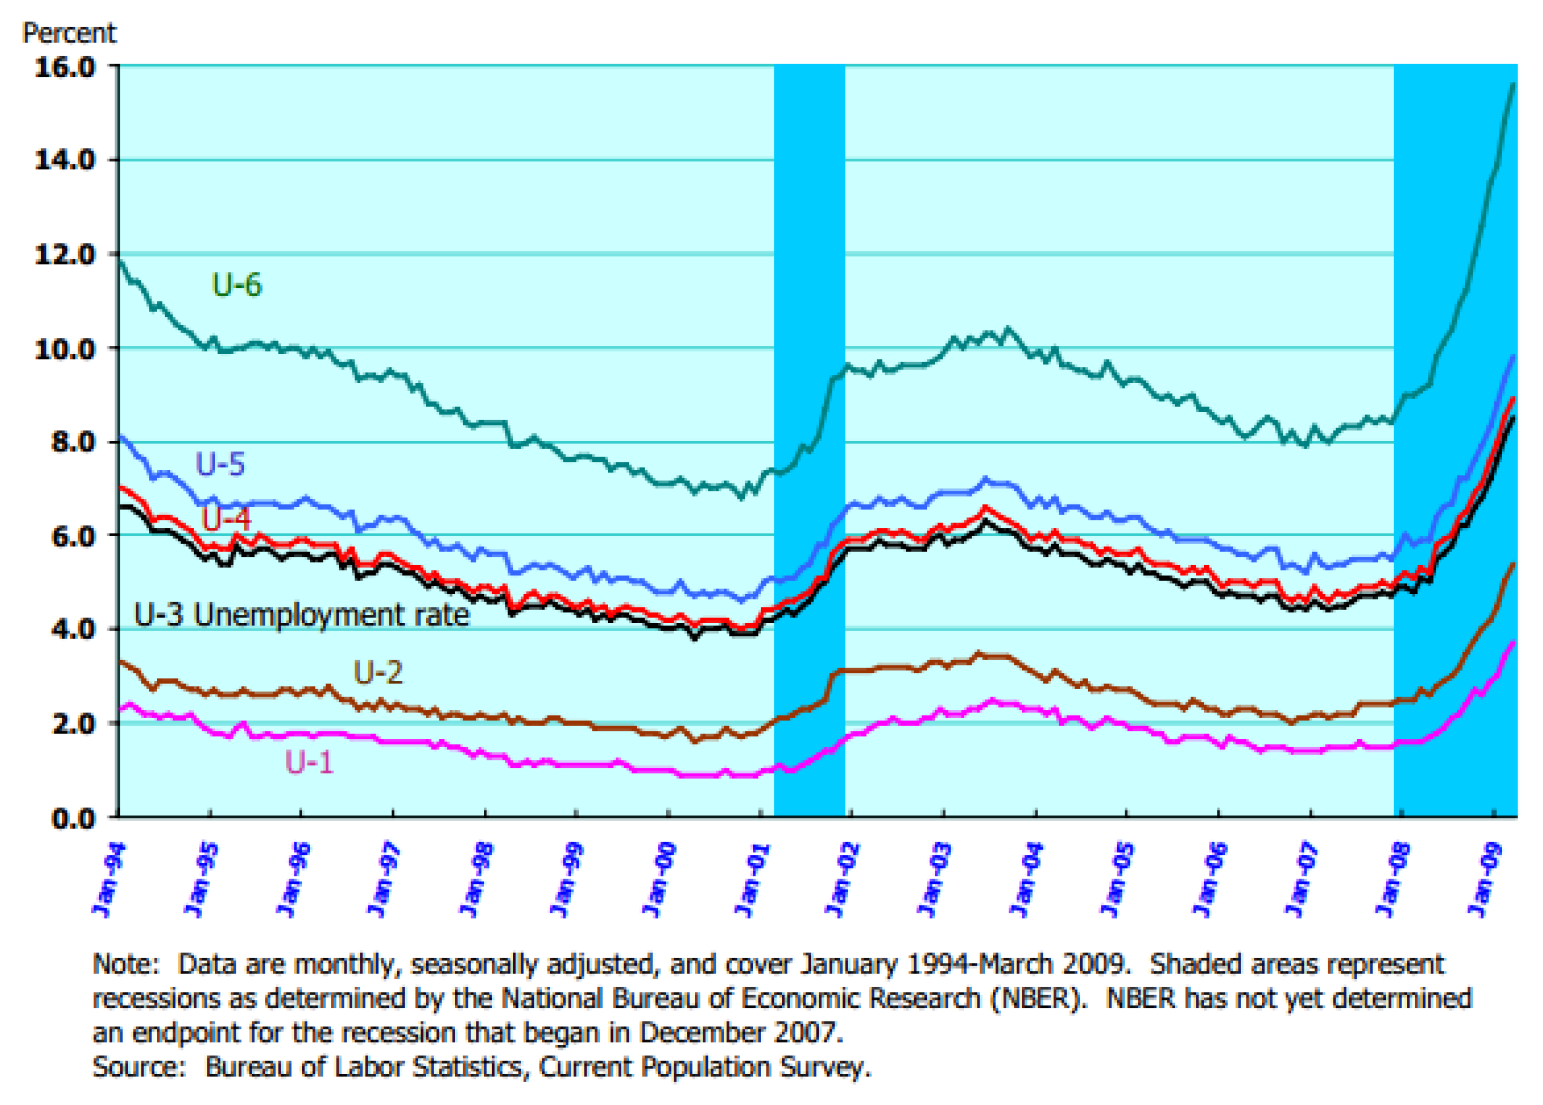
\includegraphics[scale=.3]{01C_5.png}
		\caption{Alternative Measures of Unemployment, 1994-2009}
	\end{figure}
\end{frame}

\begin{frame}{Unemployment}
\begin{exmp}
	Consider the town of Waxhaw described in the previous example. 	If we decide to change the definition of unemployment so that we counted all discouraged or marginally attached workers as ``unemployed,'' what would be the new unemployment rate?
\end{exmp}
\ddp{\pause $U' = 1,500 \Rightarrow LF' = 9000 \Rightarrow UR' = 1,500/9,000 = 16.7\%$}
\end{frame}

\begin{frame}{Unemployment}
\begin{itemize}
	\item \defn{Natural Rate of Unemployment:} The normal rate of unemployment around which the unemployment rate fluctuates.
	
	\item \defn{Cyclical Unemployment:} The deviation of unemployment from its natural rate. Generally an issue with the demand for labor.
	
\end{itemize}
\end{frame}

\begin{frame}{Unemployment}
\begin{itemize}
	\item The natural rate of unemployment is comprised of two forms of unemployment:
	\begin{enumerate}
		\item \defn{Frictional unemployment:} Unemployment that results because it takes time for workers to search for jobs.
		\item \defn{Structural unemployment:} Unemployment that results because of long-lasting shocks to permanent features of an economy.
	\end{enumerate}
	
	\item Frictional unemployment is generally limited to the \dd{short run}, while structural unemployment is more \dd{long run} in nature.
\end{itemize}
\end{frame}



\begin{frame}{Unemployment}
\scriptsize
\begin{exmp}
	
	In each of the following, determine which type of unemployment is present.
	
	\begin{enumerate}
		\item Someone who recently moved to Florida due to its warmer climate will have to spend some time looking for a job. 
		\item A worker repairing VHS cassette tapes was laid off because most customers have started using DVD players. 
		\item Natalie, a highly trained construction worker, lost her job when the recession began. He is looking for work, but the demand for labor in the industry is still low.
	
		\item Curtis has looked to work as an accountant for some time. While the demand for accountants doesn't seem to be decreasing, there seems to be more people applying than there are jobs available. 
		
	\end{enumerate}
\end{exmp}

\ddp{\pause Frictional \\
\pause Structural \\
\pause Cyclical \\
\pause Structural}
\end{frame}

\begin{frame}{Readings and Assignments}
\begin{itemize}
	\item Today: Mankiw Ch. 28
	\item Next time: Mankiw Ch. 29
	\item Problem Set 5, section 4
\end{itemize}
\end{frame}

\end{document}